%% TOMLTransformers - IEEE UEMCON 2026 submission
%% DOUBLE-BLIND: no author names, affiliations, funding, or repository URLs
%% until the camera-ready version. Prior work in the TOML series is cited in
%% the third person; never write "our previous work".
%%
%% Figures are produced by scripts/make_figures.py, which refuses to emit
%% anything unless its lineage gate reproduces the committed fit artifacts.
%% Regenerate before final compile; see paper/figures/figures_manifest.json
%% for the commit each figure was drawn at.

\documentclass[conference]{IEEEtran}
\IEEEoverridecommandlockouts

\usepackage{cite}
\usepackage{amsmath,amssymb,amsfonts}
\usepackage{graphicx}
\usepackage{textcomp}
\usepackage{xcolor}
\usepackage{booktabs}
\usepackage{url}

\graphicspath{{figures/}}

\def\BibTeX{{\rm B\kern-.05em{\sc i\kern-.025em b}\kern-.08em
    T\kern-.1667em\lower.7ex\hbox{E}\kern-.125emX}}

\begin{document}

\title{Transistor-Level Energy Modeling of Transformer\\Inference: Prefill/Decode Phase Separation and\\Cross-Architecture Transfer}

\author{\IEEEauthorblockN{Anonymous Submission}
\IEEEauthorblockA{\textit{Author names and affiliations omitted}\\
\textit{for double-blind review}}}

\maketitle

\begin{abstract}
Floating-point operation counts remain the default proxy for inference energy
despite ignoring the memory traffic that dominates it. Transistor-Operation
(TO) models replace that proxy with a physically grounded one but have been
validated only on convolutional, recurrent and tree-based architectures. We
present a transistor-level energy model for transformer inference that
decomposes energy by execution phase, accounts for KV-cache traffic and
attention-kernel choice, and is calibrated against hardware energy counters.
On an RTX 4090 the model is selected by AIC among ten forms over 296
measured configurations and attains a held-out $R^2$ of 0.987. The central
result is a phase separation: the ratio of memory to compute energy differs
by 4x to 40x between prefill and decode, and the separation reproduces on two
GPU architectures and under two estimators. A pre-registered transfer test on
an A100, with acceptance bands frozen before any result was examined, shows
the measurement methodology transfers within 0.6\% and decode energy for
7B-class models is predicted within 6\% at a 4.7x extrapolation in parameter
count. Two device-level priors do not transfer. The assumed half-precision
arithmetic cost is contradicted by a measured fp32/fp16 energy ratio of 7.4
against an analytic model ceiling of 3.03, and residual error depends on the
GPU operating point, for which the frozen model has no term. Both are
identified and quantified on both platforms. The pre-registration,
measurement data and analysis are released.
\end{abstract}

\begin{IEEEkeywords}
energy modeling, transformer inference, GPU power measurement, transistor
operations, prefill and decode, cross-architecture transfer, pre-registration
\end{IEEEkeywords}

\section{Introduction}

Machine learning inference is a growing share of datacenter electricity
demand; the International Energy Agency projects datacenter consumption to
roughly double between 2025 and 2030, with AI the dominant driver
\cite{iea2026}. The decisions that set this demand, which model to deploy,
at what precision, on which accelerator, are routinely made on
floating-point operation counts.

FLOPs are a poor energy proxy for a physical reason. Horowitz
\cite{horowitz2014} measured per-operation energy at 45\,nm and found a
range of four orders of magnitude, from 0.1\,pJ for a 32-bit integer add to
over 1{,}000\,pJ for a DRAM access. FLOPs count within a narrow band of that
range and omit the expensive entries. Data movement dominates inference
energy on modern accelerators \cite{sze2017}, so a metric blind to memory
traffic is blind to most of the energy.

Transistor-Operation (TO) models express cost in units of switching events
and calibrate a few coefficients against measured energy. Li, Tsourdos and
Guo \cite{li2024} established the approach for deep learning; Syed et al.
\cite{toml2026flairs} extended it into the TOML framework, adding metrics
including the Memory-Compute Energy Ratio (MCER) and reporting $r^2 =
0.961$ across seven architectures. Later work applied the framework to
containerized multi-tenant deployments \cite{tomlcloud2026} and to signal
processing \cite{tomlsignals2026}. None covers transformers, and a vision
paper in the same line names transformer validation as the most pressing
open gap \cite{tomlvision2026}.

The gap is structural, not just one of coverage. A transformer request runs
in two regimes. Prefill processes the prompt in parallel and is
arithmetically dense. Decode emits one token per step, does little
arithmetic, and streams the whole KV cache from memory every step. A model
assigning one energy character to ``transformer inference'' cannot describe
both. LLMCO$_2$ \cite{llmco2}, a learned estimator, found the same thing
empirically: separating prefill and decode features improved its accuracy by
32\%. What has been missing is a physically grounded account of why the
phases differ and by how much.

Contributions:

\begin{enumerate}
\item A transistor-level energy model for transformer inference
(Section~\ref{sec:model}) that counts TOs by execution phase, accounts for
KV-cache traffic, standard versus fused attention kernels and precision, and
separates kernel dispatch from computation. The form is selected by AIC
among ten candidates over 296 measured configurations on an RTX 4090 and
attains a held-out $R^2$ of 0.987.

\item A measurement methodology (Section~\ref{sec:method}) with a GPU
hardware energy counter primary and two cross-checks. Instrument agreement is
a function of window length, degrading below roughly 0.5\,s, and the 20\,Hz
sampling rate used in earlier TOML work under-reads energy by 24\%.

\item The prefill/decode phase separation (Sections~\ref{sec:results4090}
and \ref{sec:transfer}): MCER differs by 4x to 40x between the two phases,
on both Ada and Ampere, under both estimators considered.

\item A pre-registered cross-architecture transfer test
(Section~\ref{sec:transfer}), with acceptance bands for four hypotheses
frozen and committed before any A100 result was examined. The methodology
transfers within 0.6\% and 7B-class decode energy is predicted within 6\% at
a 4.7x extrapolation in parameter count.

\item Identification and quantification of the two device-level priors that
do not transfer (Section~\ref{sec:mechanism}). The model form bounds the
fp32/fp16 energy ratio at 3.03 for any non-negative coefficients; the A100
measures a median of 7.4 with no pair below the bound. The cause is
precision-dependent execution-unit routing, and the same prior is also
unsupported, less severely, on the consumer part. Separately, residual error
depends on the GPU operating point, for which the frozen model has no term.
\end{enumerate}

All pre-registered outcomes are reported as they fell, including the three
that failed their bands. Section~\ref{sec:prereg} gives the protocol,
Section~\ref{sec:baselines} the baseline comparison, and
Section~\ref{sec:discussion} argues that each failure localizes a named
physical mechanism a transferable model must represent.

\section{Background and Related Work}
\label{sec:related}

\subsection{From FLOPs to Transistor Operations}

Horowitz \cite{horowitz2014} gives the reference per-operation energies and
Sze et al. \cite{sze2017} trace the consequence for accelerator design: data
movement, not arithmetic, sets the energy budget of DNN inference.
Garc\'ia-Mart\'in et al. \cite{garciamartin2019} survey estimation methods
and document the gap between proxies and measurement. Li, Tsourdos and Guo
\cite{li2024} introduced the transistor-operation model, mapping network
operations to switching events anchored to the 45\,nm figures. TOML
\cite{toml2026flairs} added architecture-specific coefficients and six
metrics, of which MCER is used directly here. The containerized extension
\cite{tomlcloud2026} showed thermal state and co-location break the
fixed-conditions assumption; the signal processing extension
\cite{tomlsignals2026} introduced a dispatch term and reached $r^2 \geq
0.947$ on two GPUs. This paper inherits the dispatch term and MCER and adds
the transformer-specific structure neither has.

\subsection{Energy and Carbon Models for LLM Inference}

LLMCarbon \cite{llmcarbon} projects end-to-end carbon for dense and
mixture-of-experts models but targets training and treats inference with a
coarse utilization model. LLMCO$_2$ \cite{llmco2} is the closest work to
this one: it predicts inference carbon with a graph neural network over
kernel graphs and reports a 67\% improvement over prior estimators. Two of
its findings support this paper's premise. Separating prefill and decode
features raised its accuracy 32\%, and a roofline node feature added 11.3\%
by improving transfer across GPU types.

The approaches differ in kind. LLMCO$_2$ learns a mapping from a corpus of
measurements; the model here is analytic, derived from the architecture's
structure, with four coefficients fitted by non-negative least squares.
That trades expressive power for interpretability, and the trade is visible
in the results: where the analytic form is wrong, it is wrong in a way that
names a mechanism, where a learned residual would have absorbed it.

\subsection{Measurement Tools and Analytic Accelerator Models}

CodeCarbon \cite{codecarbon}, carbontracker \cite{carbontracker} and Green
Algorithms \cite{greenalgorithms} estimate energy from TDP and elapsed
time, inheriting the uniform-cost assumption. Zeus \cite{zeus} measures GPU
energy directly and is the third instrument here. Luccioni et al.
\cite{luccioni2023} report measured energy for a large model lifecycle.
Accelergy \cite{accelergy} and Timeloop \cite{timeloop} estimate
accelerator energy from architectural descriptions at finer granularity than
attempted here, but require a hardware model of the target rather than a
handful of calibration measurements.

\section{A Transistor-Level Model of Transformer Inference}
\label{sec:model}

\subsection{Cost Units}

A transistor operation is a unit of switching cost anchored to 45\,nm
circuit measurements \cite{horowitz2014}; following TOML, $1\,\mathrm{TO}
\approx 1\,\mathrm{fJ}$, so an FP32 fused multiply-add at 4.6\,pJ costs
5{,}000\,TOs. The cost table used here charges 5{,}000 TOs per MAC, 50 per
comparison, 20{,}000 per GELU, 23{,}100 per SiLU and 18{,}000 per exp or
softmax element. Memory is charged per 32-bit word: 5{,}000 TOs on-chip,
and off-chip at the vendor pJ/bit figure for the device's memory technology,
240{,}000 for the GDDR6 on the RTX 4090 Laptop part and 192{,}000 for the
HBM2E-class memory on the A100 \cite{a100datasheet}.

TO counts are workload properties, derived analytically and identical on
both platforms. The mapping to joules is deferred entirely to fitted
coefficients. The model is therefore falsifiable in a specific way: if a
coefficient fitted on one device fails to transfer, the discrepancy
localizes to the term it multiplies.

Precision enters twice. Reduced precision lowers the arithmetic cost of a
MAC by an asserted multiplier, 0.33 for fp16 against fp32, and
independently halves the number of 32-bit words moved, since an fp16
element occupies two bytes. The first is a prior about execution units; the
second follows from data layout. Section~\ref{sec:mechanism} turns on the
distinction.

\subsection{Phase Decomposition}

TOs are counted per layer from seven primitives: normalization, QKV
projection, the attention core, KV-cache write, KV-cache read, output
projection and the feed-forward block. Attention is counted according to the
kernel dispatched. A standard implementation materializes the $s \times s$
score matrix off-chip; a fused kernel of the FlashAttention family
\cite{flashattention} does not, and its scores are charged on-chip. The
difference is orders of magnitude at long context, and FLOP counts cannot
express it, since both kernels perform the same arithmetic.

The structural difference between phases is the KV cache. A prefill layer
has no cache read. A decode layer at context $c$ reads the $c-1$ cached key
and value vectors every step. For $n_{kv}$ key-value heads of dimension
$d_h$, generating $k$ tokens after a prompt of length $s$ moves

\begin{equation}
W_{\mathrm{KV}} = 2 n_{kv} d_h \sum_{t=1}^{k} (s + t - 1)
= 2 n_{kv} d_h \left( ks + \tfrac{k(k-1)}{2} \right)
\label{eq:kvtraffic}
\end{equation}

elements per layer, while decode arithmetic is dominated by the projections
and feed-forward block, $O(d^2)$ and independent of context. The ratio of
memory traffic to arithmetic grows linearly in context throughout decode; in
prefill both grow together. Equation~\ref{eq:kvtraffic} is the analytic
origin of the phase separation measured in Section~\ref{sec:results4090}.

A decode configuration cannot be measured in isolation, since a decode step
needs a populated cache. Each decode measurement is a composite execution:
one prefill over the prompt, then $k$ generated tokens with context growing
by one each step. Predicted TOs are summed over the same composite and the
regression target is energy per composite execution. A units gate asserts
this correspondence on every fit.

\subsection{Regression Form and Model Selection}

Predicted energy is linear in a small coefficient vector:

\begin{equation}
\hat{E} = \alpha_{\mathrm{mac}} T_{\mathrm{mac}}
        + \alpha_{\mathrm{nl}} T_{\mathrm{nl}}
        + \alpha_{\mathrm{sram}} T_{\mathrm{sram}}
        + \alpha_{\mathrm{hbm}} T_{\mathrm{hbm}}
        + \alpha_{d} N_{d} + \epsilon
\label{eq:m8}
\end{equation}

with $N_d$ the number of CUDA kernel launches and $\epsilon$ an intercept.
All coefficients are non-negative and fitted by NNLS; the constraint is
physical, since more computation, data movement or dispatch cannot reduce
energy. Equation~\ref{eq:m8} is one of a nested family of ten forms, from
$M_0$, a single term on total TOs equivalent to calibrated FLOP counting,
through progressively finer separations. Selection is by AIC on the RTX
4090 data, after which the form is frozen. No re-selection is performed on
the second platform.

Each form is fitted under two losses. Absolute NNLS minimizes squared error
in joules and is dominated by the largest configurations in a dataset
spanning four orders of magnitude. The relative estimator R1 minimizes
squared relative error and weights every configuration equally. Which is
primary is declared in advance per platform.

\subsection{The Memory-Compute Energy Ratio}

Following \cite{toml2026flairs}, MCER is fitted memory energy over fitted
compute energy:

\begin{equation}
\mathrm{MCER} =
\frac{\alpha_{\mathrm{sram}} T_{\mathrm{sram}} + \alpha_{\mathrm{hbm}} T_{\mathrm{hbm}}}
     {\alpha_{\mathrm{mac}} T_{\mathrm{mac}} + \alpha_{\mathrm{nl}} T_{\mathrm{nl}}} .
\label{eq:mcer}
\end{equation}

Values above unity indicate a memory-dominated regime. MCER is computed from
fitted coefficients and inherits any estimator dependence in the fit.

\subsection{A Falsifiable Structural Prediction}
\label{sec:ceiling}

The precision priors imply a bound testable without fitting. For two
configurations identical in shape but differing in precision, the MAC term
scales between fp32 and fp16 by $1/0.33 = 3.03$, the memory terms by $4/2
= 2.0$ since word counts halve, and the dispatch and intercept terms by 1.0.
The predicted energy ratio is a non-negatively weighted mean of 3.03, 2.0
and 1.0:

\begin{equation}
1.0 \leq \frac{\hat{E}_{\mathrm{fp32}}}{\hat{E}_{\mathrm{fp16}}} \leq 3.03
\qquad \text{for all } \alpha \geq 0 .
\label{eq:ceiling}
\end{equation}

No refit of Equation~\ref{eq:m8} on any device can produce a matched-shape
precision ratio above 3.03. Section~\ref{sec:mechanism} measures that ratio
on both platforms.

\section{Measurement Methodology}
\label{sec:method}

\subsection{Three Instruments}

Every configuration is measured three ways. Instrument~A integrates sampled
board power from \texttt{nvmlDeviceGetPowerUsage} at 100\,Hz by the
trapezoid rule over recorded timestamps, minus a per-point idle baseline.
Instrument~B reads the on-die energy accumulator
\texttt{nvmlDeviceGetTotalEnergyConsumption}, differenced across the window
and corrected by an equal-duration idle reading. Instrument~C is Zeus
\cite{zeus}.

Instrument~B is primary: a hardware accumulator integrates in the device at
a rate no host sampler can match. A is a methodologically distinct
cross-check and C an independent-codebase check. B and C agree to twelve
significant figures because Zeus reads the same accumulator; their
agreement validates windowing and bookkeeping, not the counter. A is the
only independent physical path.

\subsection{Instrument Characterization}

Earlier TOML work sampled power at 20\,Hz. A rate sweep on a thermally
settled 3\,s window shows 20\,Hz integrating 24.4\% below the hardware
counter, 7.1\% at 50\,Hz, and 7.1\% to 8.3\% through 100 and 200\,Hz. We
sample at 100\,Hz; the sampler saturates on our host near 96\,Hz, and the
residual plateaus rather than closing. At 100\,Hz the in-process sampler
reports 162.9\,W mean power and an out-of-process \texttt{nvidia-smi} logger
163.7\,W on the same window, ruling out interpreter contention; the
accumulator implies 177.7\,W on a part with a 175\,W sustained limit. The
residual is a sampled-power versus accumulator offset, and the accumulator
is the more plausible reading.

Agreement is a function of window length, and below roughly half a second
both readings degrade. On a 0.25\,s window A and B disagree by 36\% to
94\%, and B itself returns 33.5, 35.5, 52.1 and 37.5\,J for identical work
across repeats, the largest implying 209.6\,W on a 175\,W part. The harness
therefore sizes every window to a 4.0\,s floor by rescaling inner
iterations. Across all 296 RTX 4090 configurations the shortest achieved
window is 4.001\,s and none is flagged short. The pre-registered
configuration recorded a 2.0\,s floor; the harness enforced 4.0\,s, a
divergence in the conservative direction not amended at the time.

\subsection{Thermal Control and Replication}

Before each point the harness waits for GPU temperature stable within $\pm
1\,^{\circ}$C over 5\,s; all 296 configurations settled. A 3\,s per-point
idle measurement is subtracted, since idle drifts across a multi-hour suite.
Clock locking is refused by the laptop part, so achieved clocks are logged
per point and used in Section~\ref{sec:mechanism}. Each point has five
physical replicates, escalated to ten when a 5\% CV gate trips; 162 of 296
points escalated. Reproducibility differs by instrument: B has median CV
1.89\%, 90th percentile 4.36\%, and 94\% of points inside the gate; A has
median CV 8.90\% and exceeds the gate on 99\% of points. A, not the primary,
triggers nearly every escalation.

\subsection{Agreement Outcome}

The pre-registered target was a pooled median pairwise agreement within
5\%. Fig.~\ref{fig:f1} shows per-point A-B agreement against measured energy
on both platforms. The pooled median is 4.80\% on the RTX 4090 and 0.60\% on
the A100; median B-C agreement is 0.000\% for the reason above.

\begin{figure}[t]
\centering
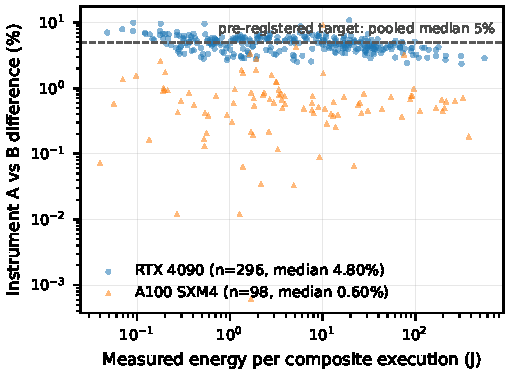
\includegraphics[width=\columnwidth]{f1_instrument_agreement.pdf}
\caption{Per-point agreement between sampled-power integration (A) and the
hardware energy counter (B) against measured energy per composite
execution. The pre-registered target constrains the pooled median, not
individual points. Achieved medians: 4.80\% (RTX 4090, $n=296$) and 0.60\%
(A100, $n=98$).}
\label{fig:f1}
\end{figure}

\subsection{Hardware}

RTX 4090 Laptop GPU (Ada Lovelace, GDDR6, 16\,GB, 175\,W sustained) on an
i9-14900HX under Windows 11, CUDA 12.4; A100-SXM4-40GB (Ampere, HBM2E-class,
400\,W) on a rented Linux instance, CUDA 13.0. The two differ in
architecture, memory technology, process node, power envelope, host CPU and
operating system.

\section{Pre-Registration and Experimental Design}
\label{sec:prereg}

A model fitted, inspected and adjusted will describe any dataset. Because
this paper reports successes and failures, the distinction was fixed before
the results existed. Every analytical decision below was written into a
dated document and committed before the corresponding numbers were
computed; the committed artifacts record the commit at which each fit ran.

\subsection{RTX 4090}

The fit plan was committed on 2026-07-20, before any fitting code existed.
It fixed the regression target as instrument~B energy per composite
execution; a phase-by-phase execution boundary table verified against the
workload source; the mapping from configuration to TO features; the
dispatch count definition; a stratified 80/20 train/test split at a recorded
seed; AIC selection on the training split among $M_0$ through $M_9$;
absolute NNLS primary with R1 as a pre-specified robustness report; the
baseline set; and Wilcoxon signed-rank tests with Holm correction at
$\alpha = 0.05$. The extrapolation hypothesis was ambiguous between two
readings, so both were declared and both computed: E1 trains on
forward-phase points at sequence dimension at most 1024 and predicts
held-out models at 2048; E2 trains on all phases and predicts all held-out
points at 2048. The band for both was 25\% held-out MAPE.

The first fit run produced $R^2 \approx 0$, an intercept near 539\,J and
negative per-token energies: the stored per-execution fields were per
repeat window, containing \texttt{inner\_iters} composite executions, and
the target had been built as though per execution. The run was discarded
before any result was accepted, the target corrected, and a permanent
consistency gate added that cross-checks the derived target against an
independently stored per-unit field on every record.

\subsection{A100}

The transfer experiment was pre-registered in a dated amendment committed on
2026-08-10, before the instance was provisioned. It fixed the grid
mechanically, using the same builder as the 4090 sweep: 84 shared points
mirroring the 4090 strata, 10 extension points at 7B scale, and 4
descriptive spot cells excluded from every fit and test. It declared R1
primary on this platform with absolute NNLS secondary, and froze the $M_8$
form with no re-selection permitted. Four hypotheses were registered with
bands recorded the same day (Table~\ref{tab:prereg}). The T1 band mirrors
the extrapolation band given an R1 full-data MAPE of 18.2\% on the 4090;
the T2 band is looser because cross-platform transfer is harder than
on-platform refit.

\begin{table}[t]
\caption{Pre-registered hypotheses, bands adopted 2026-08-10 before any A100
measurement. Bands are held-out MAPE except T0.}
\label{tab:prereg}
\centering
\small
\begin{tabular}{llc}
\toprule
Test & What it tests & Band \\
\midrule
T0 & Instrument agreement transfers & 5\% \\
T1 & On-platform refit quality & 25\% \\
T2 & Coefficient transfer, one global scale & 30\% \\
T3 & Extrapolation to 7B-class models & 30\% \\
\bottomrule
\end{tabular}
\end{table}

T2 is the strictest test. The 4090 coefficient vector is frozen; A100
features use the A100 memory tier; a single global scalar is fitted on
eight frozen calibration cells spanning size, regime and model family; the
verdict is the error on the remaining 76 points. Zero-shot transfer with the
scalar forced to unity is reported alongside. T0 through T3 test distinct
claims and are reported against their own bands with no multiplicity
correction across them.

One ambiguity surfaced after freezing: two sections of the amendment implied
different members of the T2 calibration set for one encoder-decoder cell. It
was resolved on 2026-08-17 by a structural rule, before the T2 result was
computed, and a sensitivity companion over the alternative readings is
reported; the verdict is unchanged under all of them.

Results are labeled confirmatory only if pre-registered in the form
reported. Post-verdict analyses, including the precision-split model of
Section~\ref{sec:mechanism}, are labeled exploratory in text and figure
legends, carry no verdict authority, and would require a fresh
pre-registration on new data to establish.

\section{Results: RTX 4090}
\label{sec:results4090}

The frozen dataset is 296 configurations over 14 models: five decoder-only
from DistilGPT2 to GPT-2-XL, five encoder-only including two vision
transformers, four encoder-decoder. Prefill and encode sweep sequence length;
decode sweeps context with 64 generated tokens; encoder-decoder phases use
two coordinated sub-sweeps anchored at 1024. All configurations are measured
at fp16 and fp32, and an attention sub-sweep measures the same workloads
under standard and fused kernels. All 296 points measured.

\subsection{Model Selection}

Table~\ref{tab:selection} reports the pre-registered selection on the
stratified split. $M_8$ is selected by AIC with held-out $R^2$ 0.987. $M_9$,
adding a fused-sequential term, ties on fit and loses on the parameter
penalty; no fused-sequential kernels exist in these workloads, so the term is
inert and the degeneration was anticipated in the plan. Splitting memory
into on-chip and off-chip tiers ($M_5$ over $M_1$) is the largest single
AIC improvement and adding dispatch ($M_8$ over $M_7$) the second. $M_0$,
equivalent to calibrated FLOP counting, is last by AIC.

\begin{table}[t]
\caption{Model selection on the RTX 4090, stratified 80/20 split, absolute
NNLS.}
\label{tab:selection}
\centering
\small
\begin{tabular}{lccrr}
\toprule
Model & $k$ & $R^2_{\mathrm{test}}$ & MAPE$_{\mathrm{test}}$ & AIC \\
\midrule
$M_8$ split + dispatch & 6 & \textbf{0.987} & 88.3\% & \textbf{1038.9} \\
$M_9$ full & 7 & 0.987 & 88.3\% & 1040.9 \\
$M_5$ mem split & 4 & 0.985 & 92.9\% & 1067.8 \\
$M_7$ full split & 5 & 0.985 & 92.7\% & 1069.8 \\
$M_3$ dispatch & 4 & 0.985 & 63.5\% & 1084.1 \\
$M_1$ comp + mem & 2 & 0.971 & 52.7\% & 1149.8 \\
$M_0$ FLOP-equivalent & 1 & 0.972 & 47.9\% & 1150.5 \\
\bottomrule
\end{tabular}
\end{table}

\subsection{The Two Estimators}

Table~\ref{tab:selection} shows the model with the highest $R^2$ having a
held-out MAPE near 90\%, and $M_0$, worst by AIC, the lowest MAPE.
Fig.~\ref{fig:f2} resolves this. Under the absolute fit, points cluster on
the identity line above roughly 10\,J and are over-predicted below 1\,J:
squared error in joules is set by the largest configurations, so the fit
describes them at the expense of the small ones, and MAPE, weighting every
point equally, records the damage. Under R1 the small configurations fall
onto the line, $R^2$ drops to 0.924 and MAPE falls to 18.2\%. This is
heteroscedasticity over four orders of magnitude, not a defect of the form;
it is why both estimators were pre-registered and why R1 was made primary
for the second platform. The absolute figures were primary here and are
reported as such.

\begin{figure*}[t]
\centering
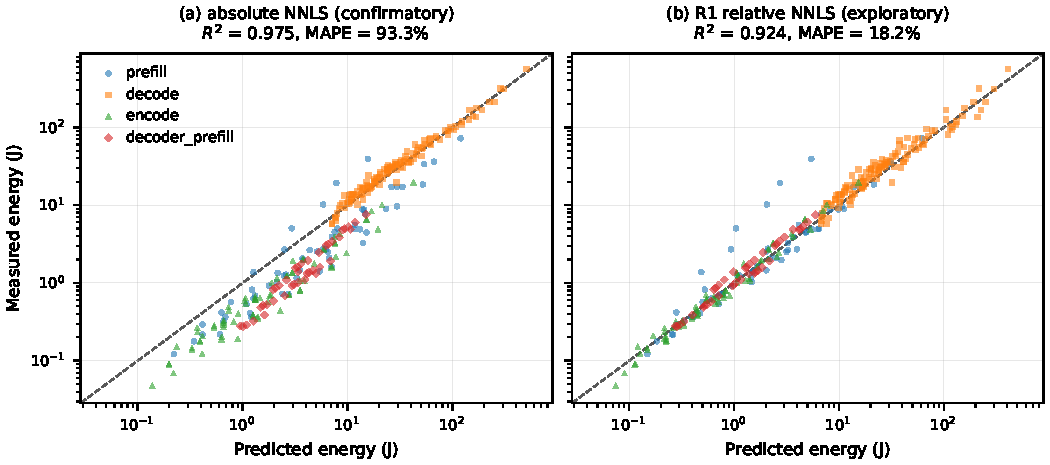
\includegraphics[width=\textwidth]{f2_4090_measured_vs_predicted.pdf}
\caption{Measured against predicted energy on the RTX 4090, $M_8$, all 296
configurations. (a)~Absolute NNLS, the pre-registered primary: the fit is
anchored by the largest configurations and over-predicts small ones.
(b)~The relative estimator R1, pre-registered as a robustness report.}
\label{fig:f2}
\end{figure*}

Under R1 over all 296 points, $\alpha_{\mathrm{mac}} = 3.44$,
$\alpha_{\mathrm{hbm}} = 7.41$ and $\alpha_{\mathrm{sram}} = 26.9$\,fJ/TO,
$\alpha_d = 0.76$\,mJ per launch, with the nonlinear coefficient and
intercept at zero. The nonlinear term is zeroed under both estimators; its
TO counts are collinear with the MAC counts on this grid, so the cost
table's nonlinear entries are untested rather than confirmed. The effective
off-chip cost, $\alpha_{\mathrm{hbm}} \times 240{,}000$, is 1.78\,nJ per
word against the 0.24\,nJ vendor prior, a factor of 7.4 that
Section~\ref{sec:transfer} shows is not constant across devices.

\subsection{The Prefill/Decode Phase Separation}
\label{sec:phasesep4090}

MCER from the fitted coefficients (Fig.~\ref{fig:f5}, first two series)
shows the separation Eq.~\ref{eq:kvtraffic} predicts. Under the absolute
estimator, decoder decode has median MCER 12.6 against 3.05 for decoder
prefill, a ratio of 4.1; under R1 the medians are 10.5 and 0.43, a ratio of
24. Encoder-decoder decode against encode is 3.2 and 37 respectively. The
separation is present under both estimators: decode is more
memory-dominated than any forward phase by a wide margin. Where unity falls
differs. Under R1 every forward phase sits below MCER $= 1$ and every decode
phase above it; under the absolute estimator all phases exceed unity. We
headline the separation, which is robust, and report the crossing under the
estimator that produces it.

Measured decode energy corroborates the mechanism. Per-token decode energy,
obtained by subtracting the matched measured prefill from each composite
and dividing by 64 tokens, rises with context: for GPT-2 at fp16 from
0.156\,J at context 128 to 0.332\,J at 2048, a factor of 2.1 for a 16-fold
increase in context, with projections and feed-forward held constant.

\subsection{Pre-Registered Extrapolation}

Both declared readings were computed. E1 passes at 14.3\% against the 25\%
band; E2 fails at 50.4\% under the primary absolute estimator, 15.2\% under
the pre-specified R1 robustness report, and is recorded as a fail.

\section{Cross-Architecture Transfer to the A100}
\label{sec:transfer}

The A100 phase measured 98 configurations with zero failures, zero
out-of-memory events and zero short windows. Table~\ref{tab:verdicts}
records the four pre-registered outcomes as they fell: one pass, three
fails. The three failures share a localizable cause.

\begin{table}[t]
\caption{Pre-registered outcomes on the A100, R1 primary, instrument B,
frozen $M_8$. Absolute-NNLS companions in parentheses.}
\label{tab:verdicts}
\centering
\small
\begin{tabular}{llrrl}
\toprule
Test & Statistic & Result & Band & Verdict \\
\midrule
T0 & pooled A-B median & 0.60\% & 5\% & PASS \\
T1 & held-out MAPE, 17 pts & 35.6\% (71.7) & 25\% & FAIL \\
T2 & MAPE, 76 pts, one scalar & 52.9\% (106.7) & 30\% & FAIL \\
T3 & MAPE, 10 pts at 7B & 42.7\% (192.5) & 30\% & FAIL \\
\bottomrule
\end{tabular}
\end{table}

\subsection{T0}

Pooled A-B agreement is 0.60\% (forward 0.58\%, decode-like 0.63\%),
against 4.80\% on the 4090 and a 5\% band. The protocol, transplanted
unchanged from a Windows laptop to a Linux datacenter instance, is better
behaved on the second platform.

\subsection{T1}

Refitting the frozen form on 67 shared points and predicting the held-out 17
gives 35.6\% against 25\%. By precision and phase, held-out error is 13.7\%
on fp16 decode and 38.2\% on fp16 forward, 39.8\% and 50.3\% on the fp32
counterparts. The signs matter more than the magnitudes: fp16 forward is
over-predicted by a mean 38\% and fp32 forward under-predicted by a mean
50\%. A single $\alpha_{\mathrm{mac}}$ is pulled between two populations
with residuals of opposite sign, the signature of an arithmetic cost that
depends on precision more strongly than the 0.33 multiplier allows.
Section~\ref{sec:mechanism} takes this up. The refit also zeroes
$\alpha_{\mathrm{sram}}$ and $\alpha_d$ on the A100, leaving two
coefficients; the dispatch term vanishing is itself a transfer result,
quantified in Section~\ref{sec:split}.

\subsection{T2 and Coefficient Transfer}

With the 4090 coefficients frozen and one scale $s^\ast$ fitted on eight
calibration cells, error on the remaining 76 points is 52.9\% against 30\%,
with $s^\ast = 0.386$; zero-shot, $s = 1$, it is 105.7\%. The sensitivity
companion over the three alternative readings of the ambiguous calibration
cell gives 52.1\%, 51.9\% and 54.2\%, all failing. The breakdown again
localizes: fp16 decode transfers at 31.7\%, fp32 forward is under-predicted
by a mean 76\%. One scalar cannot reconcile a platform whose fp16 and fp32
arithmetic costs sit in a different ratio from the calibration platform's,
and the calibration set was fp16 only by design.

The pre-registered coefficient comparison (report-only) makes the same
point. Under R1, $\alpha_{\mathrm{mac}}$ transfers at 0.91 but
$\alpha_{\mathrm{hbm}}$ at 0.49; since the memory-tier priors already carry
the GDDR6-to-HBM2E ratio, the effective per-word off-chip energy is
0.70\,nJ on the A100 against 1.78\,nJ on the 4090, a ratio of 0.39 where a
correct prior would give 1.0.

\subsection{T3}

Fitting R1 on all 84 shared points and predicting the ten 7B configurations
gives 42.7\% pooled MAPE against 30\%. The per-regime breakdown is the
strongest result of the transfer study. Decode energy for LLaMA-7B and
Mistral-7B is predicted to 5.8\% MAPE, at a 4.7-fold extrapolation in
parameter count beyond the largest model in the fit and with RMSNorm,
SiLU-gated feed-forward and, for Mistral, grouped-query attention, none of
which any shared-grid model exercises. Prefill at 1024 and 4096 is
over-predicted by a mean 67.8\%, at 8192 by 66.2\%. Fig.~\ref{fig:f7} shows
the ten points. The T3 failure is entirely a prefill failure; the
memory-bound regime of Eq.~\ref{eq:kvtraffic} transfers to a model class
the fit never saw.

\subsection{The Phase Separation Reproduces}

Fig.~\ref{fig:f5} adds the A100 series. Under R1 on the A100, decoder decode
has median MCER 4.65 against 0.114 for decoder prefill, a ratio of 41;
encoder-decoder decode against encode is 5.24 against 0.044. On all six
architecture-phase groups the A100 series sits in the same order as both
4090 series, and on both platforms the crossing of unity between forward
and decode phases appears under R1. The separation is established on two
architectures, under two estimators on the first and under the
pre-registered primary on the second.

\begin{figure*}[t]
\centering
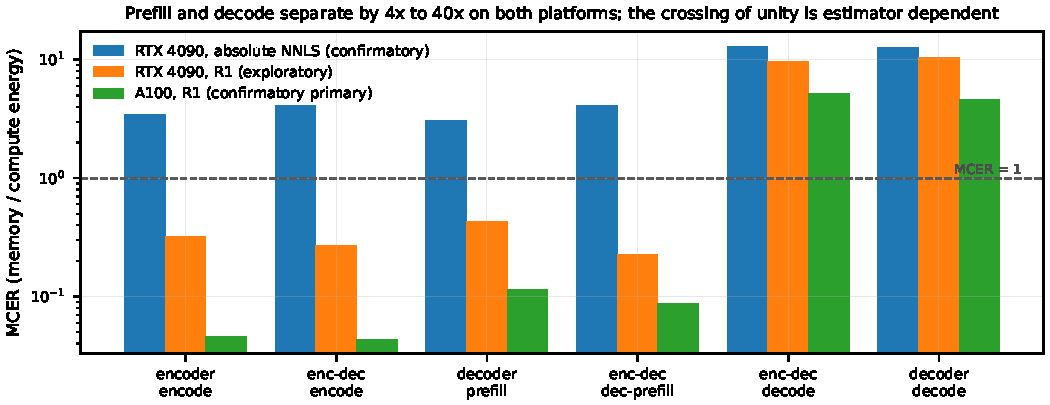
\includegraphics[width=\textwidth]{f5_mcer_phase_separation.pdf}
\caption{Median MCER by architecture and phase under three fits: RTX 4090
absolute NNLS (pre-registered primary there), RTX 4090 R1 (robustness
report), A100 R1 (pre-registered primary there). Decode exceeds every
forward phase by 4x to 40x in all three series. Where unity falls is
estimator dependent; the separation is not.}
\label{fig:f5}
\end{figure*}

The four spot cells replicate a 4090 decomposition of GPT-2 prefill at
$s=512$, fp16, across random-initialized, value-perturbed, ported-pretrained
and native-pretrained weights: weight values move energy by $-1.3\%$ to
$-3.5\%$ on the A100 (5\% to 6.5\% on the 4090), confirming random
initialization representative on the second platform.

\section{Mechanism Analysis}
\label{sec:mechanism}

Three pre-registered tests failed. The failures localize to two device-level
priors. The first two subsections use frozen data and confirmatory fits
only; the third is exploratory and labeled as such.

\subsection{The Precision Prior}
\label{sec:precision}

Section~\ref{sec:ceiling} derived, before any A100 fit, that the frozen form
cannot produce a matched-shape fp32/fp16 energy ratio above 3.03.
Fig.~\ref{fig:f4} measures that ratio directly, pairing every fp32
configuration with its fp16 twin at identical shape, kernel and phase, and
taking the ratio of instrument-B energies. On the RTX 4090, 62 forward-phase
pairs give a median of 3.24, range 2.04 to 4.11: the ceiling cuts through
the distribution and the prior is approximately right on average. On the
A100, 20 forward-phase pairs give a median of 7.43, range 6.20 to 10.20.
Every A100 pair exceeds the ceiling and the two distributions do not
overlap. No refit of the frozen form on any device could have accommodated
this; the signed residuals of Section~\ref{sec:transfer} are the fitted
consequence.

\begin{figure}[t]
\centering
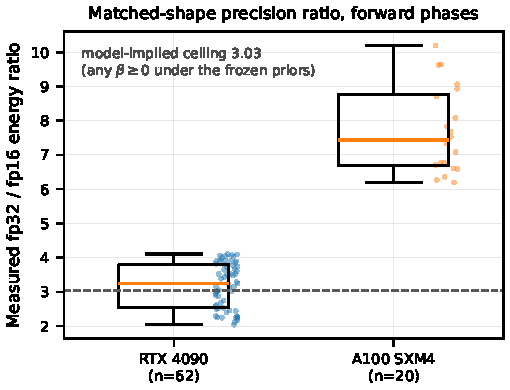
\includegraphics[width=\columnwidth]{f4_precision_ratio_by_platform.pdf}
\caption{Measured fp32/fp16 energy ratio over matched-shape forward-phase
pairs, instrument~B, both platforms. The dashed line is the analytic
ceiling of Eq.~\ref{eq:ceiling}. On the A100 no pair falls below it.}
\label{fig:f4}
\end{figure}

The mechanism is execution-unit routing. On Ampere, fp16 matrix
multiplication is dispatched to tensor cores at a dense peak of
312\,TFLOP/s, while fp32 is served by the CUDA cores at 19.5\,TFLOP/s
\cite{a100datasheet}, a 16-fold throughput gap between datapaths with
correspondingly different energy per operation. Ada also routes fp16 to
tensor cores but its fp32 path is proportionally stronger, so the gap, and
the energy ratio, is smaller. The 0.33 multiplier encodes bit-width scaling
of arithmetic cost \cite{horowitz2014}; it does not encode which silicon
executes the operation. Where precision selects the execution unit, the
multiplier is a device property and must be calibrated per device, as the
memory tier already is.

One qualification. The runner set neither the TF32 nor the fp32
matmul-precision flags, so PyTorch's default applied. On Ampere the default
can permit TF32 tensor-core execution for some operations, which would
reduce the measured ratio; that it exceeds 6 on every pair suggests the
fp32 workloads ran predominantly on the CUDA-core path. The registered
follow-up, not performed here, re-measures the matched fp32 cells with TF32
enabled; the mechanism predicts the ratio collapses toward 2 to 3.

\subsection{The Operating-Point Prior}
\label{sec:opp}

The frozen form assumes a fixed energy per transistor operation. SM clock,
board power and die temperature vary with load and power policy, and energy
per switching event varies with them. Both sweeps logged achieved median
clock and power per point. Fig.~\ref{fig:f6} groups A100 residuals by
recorded operating point. Among the fp16 flash forward cells, which hold
precision and kernel fixed, mean signed residual is $+56\%$ at 1095\,MHz and
88\,W, $+35\%$ at 1316\,MHz and 392\,W under a power cap, $+67\%$ for the 7B
cells at 1290\,MHz and 397\,W, and $+6\%$ at 1410\,MHz and 211\,W. Within a
fixed execution path the residual moves with the operating point over
roughly 60 points. The frozen form has no term for this, and no per-device
constant can supply one.

\begin{figure*}[t]
\centering
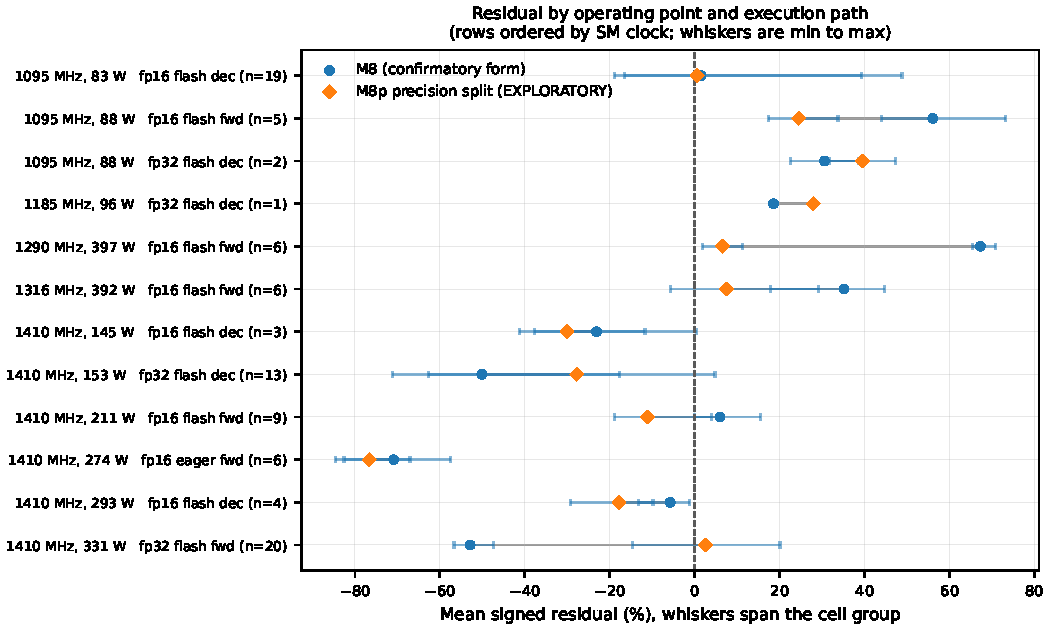
\includegraphics[width=\textwidth]{f6_operating_point_residual.pdf}
\caption{Mean signed residual on the A100 by recorded operating point and
execution path, rows ordered by SM clock, whiskers spanning each group.
Circles: confirmatory $M_8$. Diamonds: exploratory precision-split
$M_{8p}$ (Section~\ref{sec:split}), no verdict authority. Within the fp16
flash forward rows the residual tracks the operating point; the fp32 and
eager rows are set by execution path.}
\label{fig:f6}
\end{figure*}

At 1410\,MHz alone the $M_8$ residual spans $-71\%$ for the eager-attention
cells to $+6\%$ for fp16 flash forward; that spread at one clock is the
precision datapath above and, for the six eager cells, an under-prediction
of the unfused attention path on Ampere that we flag and do not pursue.

\subsection{Exploratory: Fitting the Precision Multiplier}
\label{sec:split}

The pre-registration reserved one post-verdict analysis: split the MAC
column into fp16 and fp32 columns with separate coefficients, and repeat T1
through T3 with nothing else changed. Denote this $M_{8p}$. It is
exploratory, has no verdict authority, and is reported because it tests the
mechanism claim directly.

Repeating T3 with $M_{8p}$ fitted on the 84 shared points, error on the ten
7B configurations falls from 42.7\% to 11.0\%. Fig.~\ref{fig:f7} shows the
change per point. The six prefill configurations move from $+65\%$ to
$+71\%$ under $M_8$ to $+2\%$ to $+11\%$ under $M_{8p}$; the four decode
configurations move from $-1\%$ to $-13\%$ to $-10\%$ to $-29\%$.
In-sample, fp32 forward error falls from 52.8\% to 9.1\%. The correction is
not uniform: it removes the precision confound from the arithmetic term and
exposes a smaller decode residual the confound had partly masked.

\begin{figure}[t]
\centering
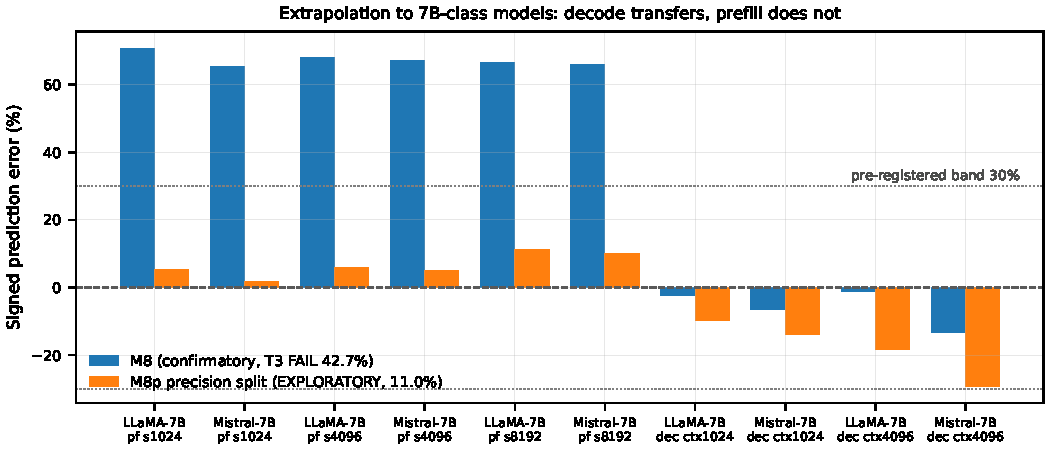
\includegraphics[width=\columnwidth]{f7_extrapolation_7b.pdf}
\caption{Signed prediction error on the ten 7B-class extension
configurations. Confirmatory $M_8$ (T3 FAIL, 42.7\%) against exploratory
$M_{8p}$ (11.0\%, no verdict authority). Dotted lines: pre-registered
$\pm 30\%$ band. Prefill collapses into the band; decode moves outward.}
\label{fig:f7}
\end{figure}

The fitted multipliers are the substantive result. On the A100 the ratio of
fitted fp16 to fp32 MAC coefficients is 0.083; refitting $M_{8p}$ on all
296 RTX 4090 points gives 0.130. The asserted 0.33 is unsupported on both
platforms; the consumer part is closer, as the mechanism predicts, but
neither is within a factor of two. Repeating T2 with $M_{8p}$ coefficients
transferred from the 4090 still fails at 52.4\%: the fitted fp32
coefficient transfers at 2.05 and the fp16 coefficient at 1.31. With the
confound removed, arithmetic energy per operation still differs between the
devices in a precision-dependent way, which is what execution-unit routing
predicts. The dispatch coefficient, present on both platforms under
$M_{8p}$, transfers at 0.0096: per-launch cost on the datacenter host is two
orders of magnitude below the laptop's.

The first written analysis of T3, recorded before the exploratory fit ran,
attributed the $+67\%$ prefill error at 7B to the operating point alone,
since those cells ran at reduced clock under a power cap. That was wrong.
The ratio of confirmatory $\alpha_{\mathrm{mac}}$ to the exploratory fp16
coefficient is $3.12/1.77 = 1.77$, which is the $+67\%$; the operating point
is a secondary contributor, the roughly 35-point spread remaining among the
fp16 forward rows after the split. The original attribution is in the
committed logbook and the correction is recorded there and here.

\section{Comparison Against Baselines}
\label{sec:baselines}

Three baselines were pre-registered: $M_0$, one coefficient on total TOs,
equivalent to calibrated FLOP counting; roofline, fitted average power
times roofline latency from vendor peak throughput and bandwidth, two
coefficients; and layerwise, one coefficient per layer type. Each is
compared against $M_8$ by one-sided Wilcoxon signed-rank test on per-point
absolute percentage error over the held-out split, Holm-corrected at
$\alpha = 0.05$. Table~\ref{tab:baselines} reports held-out MAPE and
Holm-corrected $p$ for all four on both platforms under both estimators.

\begin{table}[t]
\caption{Held-out MAPE (\%) against pre-registered baselines. RTX 4090:
main test split, 58 points; A100: T1 test split, 17 points. $M_8$ beats
layerwise under absolute NNLS on both platforms ($p_{\mathrm{Holm}} =
0.0005$ and $0.0003$); every other comparison has $p_{\mathrm{Holm}} \geq
0.43$. The last two rows give the roofline baseline's fitted average power
against each part's rated envelope.}
\label{tab:baselines}
\centering
\small
\begin{tabular}{lrrrr}
\toprule
 & \multicolumn{2}{c}{RTX 4090} & \multicolumn{2}{c}{A100} \\
\cmidrule(lr){2-3}\cmidrule(lr){4-5}
Model & abs. & R1 & abs. & R1 \\
\midrule
$M_8$ (this work) & 88.3 & 20.1 & 71.7 & 35.6 \\
$M_0$ FLOP-equivalent & 47.9 & 32.4 & 66.0 & 36.6 \\
roofline & 29.8 & 30.2 & 33.0 & 32.2 \\
layerwise & 96.5 & 24.6 & 174.1 & 39.8 \\
\midrule
roofline $P_{\mathrm{avg}}$ (W) & 378 & -- & 413 & 369 \\
rated envelope (W) & \multicolumn{2}{c}{150 to 175} & \multicolumn{2}{c}{400} \\
\bottomrule
\end{tabular}
\end{table}

On the RTX 4090 under the pre-registered absolute estimator, $M_8$ beats
only the layerwise baseline; it does not beat $M_0$ or roofline, and both
are numerically better on held-out MAPE, for the dynamic-range reason of
Section~\ref{sec:results4090}. Under R1 the ordering inverts and $M_8$
leads. On the A100 under R1, $M_8$ beats nothing, with
$p_{\mathrm{Holm}} \geq 0.43$ throughout on a 17-point split; under the
absolute companion only layerwise is beaten.

A calibrated FLOP count with one coefficient is therefore competitive with
a five-coefficient analytic model on these splits, and roofline is slightly
better on both platforms. This is consistent with Section~\ref{sec:mechanism}:
what $M_8$ adds over $M_0$ is structure, and that structure is built on a
precision prior that is wrong on the A100 and approximate on the 4090, so
the additional terms carry error as well as information. The baselines have
no precision prior to get wrong. The exploratory $M_{8p}$ results suggest
correcting it changes the comparison; establishing that needs a fresh
pre-registration.

The roofline baseline is also physically unsound on one platform. Its fitted
average power is 378\,W on the RTX 4090, roughly twice the laptop part's
envelope; on the A100 it is 369\,W under R1 against a 400\,W part. A model
can predict energy well while implying an impossible operating point,
because power and latency errors cancel. The TO
coefficients are energies per switching event and must be non-negative;
they cannot compensate this way, which costs accuracy on a small split and
buys interpretability. Section~\ref{sec:mechanism} could not have been
written from the roofline fit.

\section{Discussion and Limitations}
\label{sec:discussion}

\subsection{What Transfers and What Does Not}

Workload structure transfers; device priors do not. The quantities derived
from the architecture's definition, the phase decomposition, KV-cache
traffic and its linear growth in context, and the attention-kernel
accounting, reproduce across two GPU architectures, operating systems and
memory technologies, and the memory-bound regime they describe predicts 7B
decode within 6\% from models a fifth the size. The quantities asserted from
datatype or vendor priors, the fp16 arithmetic multiplier and the per-word
memory tier, do not transfer, and the dispatch cost differs by two orders of
magnitude between hosts.

The coefficient vector therefore divides in two. TO counts and their phase
structure can be computed once per architecture and shipped. The per-device
parameters, at least a per-precision arithmetic cost, a per-tier memory
cost and a dispatch cost, must be calibrated on each target from a small
measured set. The A100 results suggest the set can be small: 84 points, and
the exploratory refit on them predicts 7B decode and prefill within 11\%.
The operating-point dependence is harder, because it varies within a
device. A term in recorded clock or power is the natural extension and the
subject of follow-up work; LLMCO$_2$'s roofline node feature \cite{llmco2}
can be read as an empirical version of the same correction.

\subsection{On Reporting Failures}

One passed and three failed hypotheses is not a weak result. A test that
passes confirms what the model already encoded; a test that fails, and whose
failure localizes to a named term, identifies what it must additionally
encode. None of Section~\ref{sec:mechanism} exists under a protocol that
permits the form to be adjusted until it passes.

\subsection{Limitations}

Two GPUs, both NVIDIA, one consumer and one datacenter; the device-property
claim for the precision multiplier rests on two points, and a third
tensor-core generation would test it, as would the registered TF32
follow-up. The A100 test splits are small, 17 points for T1 and 10 for T3,
and the baseline comparisons there have low power. Random-initialized
weights throughout, representative of operation shapes and data movement
but not of any particular serving stack. The nonlinear term is untested by
the confirmatory fits, and the six eager attention cells on Ampere are
under-predicted by roughly four-fold and left unexplained.

\section{Conclusion}
\label{sec:conclusion}

We have presented the first transistor-level energy model of transformer
inference, decomposed by execution phase and calibrated against hardware
energy counters on two GPU architectures under a pre-registered protocol.
The central result is a phase separation: the ratio of memory to compute
energy differs by 4x to 40x between prefill and decode, follows analytically
from KV-cache traffic growing under fixed arithmetic, and reproduces on
both platforms and under both estimators. The methodology transfers within
0.6\% and decode energy at 7B scale is predicted within 6\% from models a
fifth the size.

Three pre-registered transfer tests failed, for two identifiable reasons. A
precision prior that bounds the fp32/fp16 energy ratio at 3.03 is
contradicted by every measured A100 pair, median 7.4, because precision
selects the execution unit on that device; and energy per transistor
operation depends on an operating point the frozen form does not represent.
Both are quantified on both platforms. Workload structure transfers across
hardware and device priors do not, so the latter must be calibrated per
target rather than asserted from datatype or vendor figures. The
pre-registration, measurement data, fit artifacts and figure pipeline, which
verifies every plotted number against the committed results before drawing,
are released with the paper.

\IEEEtriggeratref{3}
\bibliographystyle{IEEEtran}
\bibliography{refs}

\end{document}
